%\VignetteIndexEntry{FunciSNP Vignette}
%\VignetteDepends{}
%\VignetteKeywords{SNP Functional GWAS}
%\VignettePackage{FunciSNP}
\documentclass[a4paper]{article}
\usepackage[OT1]{fontenc}
\usepackage{Sweave}
\begin{document}

\title{Vignette\\FunciSNP: Functional Identification of SNPs with
\\Phenotype by Coincidence with Chromatin Biofeatures}
\author{Simon G. Coetzee, Suhn Rhie, Gerhard A. Coetzee and Houtan 
Noushmehr\\\\Norris Cancer Center\\Keck School of Medicine\\University
 of Southern California\\Los Angeles, USA.
}

\maketitle
\section*{Introduction}
FunciSNP assist in identifying putative functional SNP from previously
 identified GWAS SNPs (tagSNP). Using information from the 1000 genomes 
 database as well as known position of GWAS tagSNP currated for a particular 
 trait or disease, FunciSNP integrates the two data along with sequence 
 information provided by peaks identified from high-throughput sequencing. 
 FunciSNP assumes user will provide peaks identified using any available 
 ChIP peak algorithm, such as FindPeaks.

This vignette provides a 'HOW-TO' guide to setup and run FunciSNP on your 
machine. FunciSNP was developed with the idea that a user will have 
uninterupted high-speed internet access as well as a desktop machine with 
more than 4 multiple cores. If user is using a windows machine, multiple
 cores options will not work and thus total time to complete initial FunciSNP
  analysis will take longer than expected. Be sure you have uninterupted 
  computing power when using a windows machine. If using a linux machine, 
  please use 'screen' (see man screen for more information).

Using a 64bit Linux machine running 11.04 Ubuntu OS with 24G RAM and 8 cores
 connected to a academic high-speed internet port, the amount of time to 
 complete 99 tagSNP across 20 different biofeatures took less than 30 min
 to complete. We anticipate about 2 hours to complete the same analysis 
 using one core.
\section*{Load FunciSNP+other useful libraries}
\begin{Schunk}
\begin{Sinput}
> #When package is offically posted in Bioconductor, uncomment next 2 lines.
> #source("http://bioconductor.org/biocLite.R")
> #biocLite("FunciSNP");
> ## Following two packages and options() are not required to run 'FunciSNP' but 
> #will enhance the analysis experience.
> #library(setwidth); ## Automatically set the value of options("width") when the 
> #terminal emulator is resized
> #library(colorout); ## colorize R output on terminal emulators
> options(width=80);
> ##FunciSNP library and other related libraries needed.
> library("org.Hs.eg.db");
> library("gplots");
> library("gtools");
> library("ggplot2");
> library("matlab");
> library(FunciSNP);
> package.version("FunciSNP");
\end{Sinput}
\begin{Soutput}
[1] "0.1.8"
\end{Soutput}
\end{Schunk}

\section*{Identify FuncySNP using published GWAS SNPs and publicly available 
biological features (ENCODE ChIPseq peaks)}
\subsection*{FuncySNP()}
This section describes the main function of FunciSNP. 

It will identify correlated SNPs which are in linkage disequilibrium (LD) 
to a known disease associated tagSNP. It will also determine if the 
correlated SNP in LD to the tagSNP overlaps a genomic biological feature. 
Correlated SNPs are directly imported from the current public release of 
the 1000 genomes database. 1000 genomes ftp servers available for the 
1000 genomes public data: 1) National Center for Biotechnology Information 
(NCBI) ftp://ftp-trace.ncbi.nih.gov/1000genomes/; 2) European Bioinformatics
Institute (EBI) ftp://ftp.1000genomes.ebi.ac.uk/vol1/.

Correlated SNPs in LD to a tagSNP and overlapping genomic biological features 
are known as putative functional SNPs (also defined as 'FuncySNP' elsewhere in
 the package.).

As an example, we collected SNPs identified by GWAS for Glioblastoma multiforme 
(GBM). In this example, GBM includes lower grade glioma, thus the use of 'glioma'
 to label all objects.

GWAS SNPs file should be in a tab or whitespace separated file. Three 
columns are required for each GWAS tagSNP. Position, rsID, population.
Positon should be the exact postion for each rsID as determined by human
 genome build hg19 (Chromosome:Postion). rsID should contain a unique 
 rsID as determined by the 1000 genomes database for each identified GWAS
  tagSNP. Population should be a three letter code to determine original 
  ethnic population for which the associated tagSNP was identified. The 
 three letter code should be either European (EUR), Asian (ASN), African 
 (AFR), American (AMR), or All (ALL). List each tagSNP for multiple ethnic 
 population.
\begin{Schunk}
\begin{Sinput}
> ## Full path to the example GWAS SNP regions file for Glioblastoma 
> #  (collected from SNPedia on Jan 2012)
> glioma.snp <- file.path(system.file('extdata', package='FunciSNP'), 
+ dir(system.file('extdata',package='FunciSNP'), pattern='.snp$'));
> gsnp <- read.delim(file=glioma.snp,sep=" ",header=FALSE);
> gsnp;
\end{Sinput}
\begin{Soutput}
            V1        V2  V3
1 11:118477367  rs498872 EUR
2    5:1286516 rs2736100 ASN
3   9:22068652 rs4977756 EUR
4  20:62309839 rs6010620 EUR
\end{Soutput}
\end{Schunk}
Each biofeature used to identify correlated SNP should be in standard BED
 format. All biofeatures should be stored in one folder and should have 
 file extension .bed. Here is an example of three different biofeatures
  used for the glioma example.
\begin{Schunk}
\begin{Sinput}
> #glioma.snp;
> ## Full path to the example biological features BED files 
> #  derived from the ENCODE project for Glioblastoma U-87 cell lines.
> glioma.bio <- system.file('extdata',package='FunciSNP');
> list.files(glioma.bio, pattern='.bed$');
\end{Sinput}
\begin{Soutput}
[1] "knownGene.TSS.hg19.bed" "TFBS_Nrsf_U87.bed"      "TFBS_Pol2_U87.bed"     
\end{Soutput}
\begin{Sinput}
> nrsf.filename <- list.files(glioma.bio, pattern='.bed$')[2];
> Nrsf <- read.delim(file=paste(glioma.bio, nrsf.filename,sep="/"), sep="\t",
+         header=FALSE);
> head(Nrsf);
\end{Sinput}
\begin{Soutput}
    V1        V2        V3                      V4 V5 V6
1 chr5 178601706 178602140 Merged-chr5-178601923-1  0  +
2 chr5 178850156 178850592 Merged-chr5-178850374-1  0  +
3 chr5 179015119 179015553 Merged-chr5-179015336-1  0  +
4 chr7     23844     24636     Merged-chr7-24240-1  0  +
5 chr7     65601     66065     Merged-chr7-65833-1  0  +
6 chr7    128907    129421    Merged-chr7-129164-1  0  +
\end{Soutput}
\end{Schunk}
Following will take about 10 min to run.
\begin{Schunk}
\begin{Sinput}
> #glioma.bio;
> ## FunciSNP analysis, extracts correlated SNPs from the 
> #  1000 genomes db ("ncbi" or "ebi") and finds overlaps between 
> #  correlated SNP and biological features and then 
> #  calculates LD (Rsquare, Dprime, distance, p-value).
> ## Depending on number of CPUs and internet connection, this step may take 
> # some time. Please consider using a unix machine to access multiple cores.
> # glioma <- FuncySNP(snp.regions.file=glioma.snp, 
> #           bio.features.loc = glioma.bio, 
> #           bio.features.TSS=FALSE);
> # glioma;
> # summary(glioma);
\end{Sinput}
\end{Schunk}
If you decide not to run 'FuncySNP', you can call the results as
 follows. This was precompiled to provide user an example dataset to work 
 with in this tutorial.
\begin{Schunk}
\begin{Sinput}
> data(glioma);
> glioma;
\end{Sinput}
\begin{Soutput}
TagSNP List with  4  Tag SNPs and 
 778 nearby,  potentially correlated SNPs, that overlap at least one biofeature 
$`R squared: 0.1`
             Total R.squared.cuff.0.1 Percent
tagSNPs          4                  3   75.00
1kSNPs         778                 64    8.23
bio.features     3                  3  100.00

$`R squared: 0.5`
             Total R.squared.cuff.0.5 Percent
tagSNPs          4                  3   75.00
1kSNPs         778                 44    5.66
bio.features     2                  2  100.00

$`R squared: 0.9`
             Total R.squared.cuff.0.9 Percent
tagSNPs          4                  1   25.00
1kSNPs         778                 13    1.67
bio.features     2                  2  100.00
\end{Soutput}
\begin{Sinput}
> summary(glioma);
\end{Sinput}
\begin{Soutput}
TagSNP List with  4  Tag SNPs and 
 778 nearby,  potentially correlated SNPs, that overlap at least one biofeature 
Number of potentially correlated SNPs 
overlapping at least x biofeatures, per Tag SNP at an R squared of
$`R squared: 0.1 in 4 Tag SNPs with a total of `
                        bio.1 bio.2
rs4977756                   3     0
rs498872                    9     2
rs6010620                  52     9
TOTAL # CORRELATED SNPS    64    11

$`R squared: 0.5 in 4 Tag SNPs with a total of `
                        bio.1 bio.2
rs4977756                   2     0
rs498872                    2     0
rs6010620                  40     6
TOTAL # CORRELATED SNPS    44     6

$`R squared: 0.9 in 2 Tag SNPs with a total of `
                        bio.1
rs6010620                  13
TOTAL # CORRELATED SNPS    13
\end{Soutput}
\begin{Sinput}
> class(glioma);
\end{Sinput}
\begin{Soutput}
[1] "TSList"
attr(,"package")
[1] "FunciSNP"
\end{Soutput}
\end{Schunk}

\subsection*{Annotating newly identified FuncySNPs}
All known genomic features (exon, intron, 5'UTR, 3'UTR, promoter, lincRNA or in 
gene desert (intergentic)) are used to annotate each newly identified FuncySNP.
 Information described in this data.frame() is used for all summary plots, table, 
 and to output results in BED format. This step should be completed after 
 running FuncySNP().
\begin{Schunk}
\begin{Sinput}
> glioma.anno <- FunciSNPAnnotateSummary(glioma);
> class(glioma.anno);
\end{Sinput}
\begin{Soutput}
[1] "data.frame"
\end{Soutput}
\begin{Sinput}
> gl.anno <- glioma.anno;
> ## remove rownames for this example section.
> rownames(gl.anno) <- c(1:length(rownames(gl.anno)))
> dim(gl.anno);
\end{Sinput}
\begin{Soutput}
[1] 862  28
\end{Soutput}
\begin{Sinput}
> head(gl.anno); ## 
\end{Sinput}
\begin{Soutput}
  chromosome bio.feature.start bio.feature.end        bio.feature  corr.snp.id
1          5           1200710         1201809 knownGene.TSS.hg19 chr5:1200720
2          5           1200710         1201809 knownGene.TSS.hg19 chr5:1200766
3          5           1200710         1201809 knownGene.TSS.hg19 chr5:1200817
4          5           1200710         1201809 knownGene.TSS.hg19 chr5:1200946
5          5           1200710         1201809 knownGene.TSS.hg19 chr5:1200976
6          5           1200710         1201809 knownGene.TSS.hg19 chr5:1201033
  corr.snp.position tag.snp.id tag.snp.position   D.prime    R.squared p.value
1           1200720  rs2736100          1286516        NA           NA       1
2           1200766  rs2736100          1286516        NA           NA       1
3           1200817  rs2736100          1286516        NA           NA       1
4           1200946  rs2736100          1286516        NA           NA       1
5           1200976  rs2736100          1286516 1.0000000 0.0022585199       1
6           1201033  rs2736100          1286516 0.1795671 0.0004069606       1
  distance.from.tag population.count population nearest.lincRNA.ID
1            -85796              286        ASN     TCONS_00010241
2            -85750              286        ASN     TCONS_00010241
3            -85699              286        ASN     TCONS_00010241
4            -85570              286        ASN     TCONS_00010241
5            -85540              286        ASN     TCONS_00010241
6            -85483              286        ASN     TCONS_00010241
  nearest.lincRNA.distancetoFeature nearest.lincRNA.coverage
1                            -39302                 upstream
2                            -39348                 upstream
3                            -39399                 upstream
4                            -39528                 upstream
5                            -39558                 upstream
6                            -39615                 upstream
  nearest.TSS.GeneSymbol        nearest.TSS.refseq nearest.TSS.ensembl
1                SLC6A19 NM_001003841;NP_001003841     ENSG00000174358
2                SLC6A19 NM_001003841;NP_001003841     ENSG00000174358
3                SLC6A19 NM_001003841;NP_001003841     ENSG00000174358
4                SLC6A19 NM_001003841;NP_001003841     ENSG00000174358
5                SLC6A19 NM_001003841;NP_001003841     ENSG00000174358
6                SLC6A19 NM_001003841;NP_001003841     ENSG00000174358
  nearest.TSS.coverage nearest.TSS.distancetoFeature Promoter utr5 Exon Intron
1             upstream                          -990      YES   NO   NO     NO
2             upstream                          -944      YES   NO   NO     NO
3             upstream                          -893      YES   NO   NO     NO
4             upstream                          -764      YES   NO   NO     NO
5             upstream                          -734      YES   NO   NO     NO
6             upstream                          -677      YES   NO   NO     NO
  utr3 Intergenic
1   NO         NO
2   NO         NO
3   NO         NO
4   NO         NO
5   NO         NO
6   NO         NO
\end{Soutput}
\begin{Sinput}
> names(gl.anno);
\end{Sinput}
\begin{Soutput}
 [1] "chromosome"                        "bio.feature.start"                
 [3] "bio.feature.end"                   "bio.feature"                      
 [5] "corr.snp.id"                       "corr.snp.position"                
 [7] "tag.snp.id"                        "tag.snp.position"                 
 [9] "D.prime"                           "R.squared"                        
[11] "p.value"                           "distance.from.tag"                
[13] "population.count"                  "population"                       
[15] "nearest.lincRNA.ID"                "nearest.lincRNA.distancetoFeature"
[17] "nearest.lincRNA.coverage"          "nearest.TSS.GeneSymbol"           
[19] "nearest.TSS.refseq"                "nearest.TSS.ensembl"              
[21] "nearest.TSS.coverage"              "nearest.TSS.distancetoFeature"    
[23] "Promoter"                          "utr5"                             
[25] "Exon"                              "Intron"                           
[27] "utr3"                              "Intergenic"                       
\end{Soutput}
\begin{Sinput}
> summary(gl.anno[,c(1:18,20:28)]);
\end{Sinput}
\begin{Soutput}
  chromosome        bio.feature.start   bio.feature.end    
 Length:862         Min.   :  1200710   Min.   :  1201809  
 Class :character   1st Qu.: 62295044   1st Qu.: 62295926  
 Mode  :character   Median : 62326155   Median : 62337392  
                    Mean   : 65165595   Mean   : 65169512  
                    3rd Qu.: 62374564   3rd Qu.: 62376020  
                    Max.   :118531575   Max.   :118532674  
                                                           
             bio.feature           corr.snp.id  corr.snp.position  
 knownGene.TSS.hg19:372   chr11:118442863:  2   Min.   :  1200720  
 TFBS_Nrsf_U87     : 22   chr11:118443036:  2   1st Qu.: 62295889  
 TFBS_Pol2_U87     :468   chr11:118443046:  2   Median : 62327508  
                          chr11:118478342:  2   Mean   : 65167605  
                          chr20:62289690 :  2   3rd Qu.: 62375255  
                          chr20:62289873 :  2   Max.   :118532636  
                          (Other)        :850                      
     tag.snp.id  tag.snp.position       D.prime            R.squared        
 rs2736100: 96   Min.   :  1286516   Min.   :7.835e-04   Min.   :9.520e-08  
 rs4977756: 25   1st Qu.: 62309839   1st Qu.:9.338e-01   1st Qu.:7.765e-04  
 rs498872 :166   Median : 62309839   Median :1.000e+00   Median :4.501e-03  
 rs6010620:575   Mean   : 65163135   Mean   :8.995e-01   Mean   :1.258e-01  
                 3rd Qu.: 62309839   3rd Qu.:1.000e+00   3rd Qu.:2.804e-02  
                 Max.   :118477367   Max.   :1.000e+00   Max.   :9.776e-01  
                                     NA's   :4.710e+02   NA's   :4.710e+02  
    p.value           distance.from.tag population.count population
 Min.   :2.115e-163   Min.   :-100000   Min.   :286.0    ASN: 96   
 1st Qu.: 1.000e+00   1st Qu.: -19966   1st Qu.:379.0    EUR:766   
 Median : 1.000e+00   Median :  13942   Median :379.0              
 Mean   : 7.989e-01   Mean   :   4470   Mean   :368.6              
 3rd Qu.: 1.000e+00   3rd Qu.:  25290   3rd Qu.:379.0              
 Max.   : 1.000e+00   Max.   :  67371   Max.   :379.0              
                                                                   
      nearest.lincRNA.ID nearest.lincRNA.distancetoFeature
 TCONS_00010241: 96      Min.   :-265183                  
 TCONS_00015797: 25      1st Qu.: -92280                  
 TCONS_00020001:166      Median :  59111                  
 TCONS_00027984: 26      Mean   :   2073                  
 TCONS_00028269:549      3rd Qu.:  73343                  
                         Max.   : 246019                  
                                                          
 nearest.lincRNA.coverage    nearest.TSS.GeneSymbol      nearest.TSS.ensembl
 downstream:565           TNFRSF6B      :305        ENSG00000243509:305     
 inside    :  9           PHLDB1        : 86        ENSG00000019144: 86     
 upstream  :288           ZGPAT         : 68        ENSG00000197114: 68     
                          RTEL1;TNFRSF6B: 37        ENSG00000229299: 59     
                          SLC6A18       : 34        ENSG00000026036: 37     
                          (Other)       :202        ENSG00000244977: 36     
                          NA's          :130        (Other)        :271     
 nearest.TSS.coverage nearest.TSS.distancetoFeature Promoter   utr5    
 downstream:103       Min.   :-16454.0              NO :694   NO :825  
 inside    :311       1st Qu.: -3117.0              YES:168   YES: 37  
 upstream  :448       Median :   -76.0                                 
                      Mean   :   890.4                                 
                      3rd Qu.:  2305.8                                 
                      Max.   : 28781.0                                 
                                                                       
  Exon     Intron     utr3     Intergenic
 NO :776   NO :413   NO :702   NO :810   
 YES: 86   YES:449   YES:160   YES: 52   
\end{Soutput}
\begin{Sinput}
> rm(gl.anno);
\end{Sinput}
\end{Schunk}
\subsection*{Summary table used to describe newly identified FuncySNPs}
Using a specified Rsquare value (0-1) to subset the data, a table is generated 
which summarizes the total number of FuncySNPs, associated tagSNPs, and number
 of overlapping biofeatures. This will provide user a first look at the total 
 number of available FuncySNP at a particular Rsquare cutoff.
\begin{Schunk}
\begin{Sinput}
> FunciSNPtable(glioma.anno, rsq=0.5);
\end{Sinput}
\begin{Soutput}
             Total R.squared.cuff.0.5 Percent
tagSNPs          4                  3   75.00
1kSNPs         778                 44    5.66
bio.features     2                  2  100.00
\end{Soutput}
\end{Schunk}
If 'geneSum' is set to TRUE, a list of gene names is reported instead.
\begin{Schunk}
\begin{Sinput}
> FunciSNPtable(glioma.anno, rsq=0.5, geneSum=TRUE);
\end{Sinput}
\begin{Soutput}
      Gene_Names
1         CDKN2B
2          LIME1
3         PHLDB1
4       SLC2A4RG
5       TNFRSF6B
6           TREH
7          ZGPAT
8 RTEL1;TNFRSF6B
\end{Soutput}
\end{Schunk}
\subsection*{Summary of correlated SNPs overlapping biofeatures}
This function helps in determining the number of correlated SNPs overlapping 
a number of different biofeatures. This is similar to running 'summary(glioma)'
above, except now you can specifically call the function and set a 
pre-determined 'rsq' value to subset the data and thereby obtain a 
more objective and informative result.
\begin{Schunk}
\begin{Sinput}
> FunciSNPsummaryOverlaps(glioma.anno)
\end{Sinput}
\begin{Soutput}
                        bio.1 bio.2
rs2736100                  41     0
rs4977756                  12     0
rs498872                   59     3
rs6010620                 236    40
TOTAL # CORRELATED SNPS   348    43
\end{Soutput}
\end{Schunk}
Using a 'rsq' value, the output is subsetted to summarize the results with 
Rsquare values greater than or equal to 'rsq'.
\begin{Schunk}
\begin{Sinput}
> FunciSNPsummaryOverlaps(glioma.anno, rsq=0.5)
\end{Sinput}
\begin{Soutput}
                        bio.1 bio.2
rs4977756                   2     0
rs498872                    2     0
rs6010620                  40     6
TOTAL # CORRELATED SNPS    44     6
\end{Soutput}
\end{Schunk}
\subsection*{Summary of correlated SNPs for a number of different tagSNPs}
After running FunciSNPsummaryOverlaps(), the next question one would like to 
know is which correlated SNPs overlapping a number of different biofeatures 
for a number of associated tagSNP. Thus, in the example above, we have 
determined that we are interested in learning more about the correlated 
SNPs associated with 'rs6010620' and which overlap at least 2 different 
biofeatures.
\begin{Schunk}
\begin{Sinput}
> rs6010620 <- FunciSNPidsFromSummary(glioma.anno, tagsnpid="rs6010620", 
+         num.features=2, rsq=0.5)
> summary(rs6010620);
\end{Sinput}
\begin{Soutput}
  chromosome        bio.feature.start  bio.feature.end   
 Length:12          Min.   :62326155   Min.   :62330994  
 Class :character   1st Qu.:62329895   1st Qu.:62337392  
 Mode  :character   Median :62354158   Median :62355398  
                    Mean   :62351007   Mean   :62353861  
                    3rd Qu.:62370211   3rd Qu.:62371310  
                    Max.   :62371621   Max.   :62372970  
                                                         
             bio.feature    corr.snp.id corr.snp.position      tag.snp.id
 knownGene.TSS.hg19:6    rs1056441:2    Min.   :62330439   rs2736100: 0  
 TFBS_Nrsf_U87     :0    rs1291209:2    1st Qu.:62330484   rs4977756: 0  
 TFBS_Pol2_U87     :6    rs1295810:2    Median :62354704   rs498872 : 0  
                         rs1741708:2    Mean   :62352184   rs6010620:12  
                         rs6062498:2    3rd Qu.:62370732                 
                         rs6122159:2    Max.   :62372041                 
                         (Other)  :0                                     
 tag.snp.position      D.prime         R.squared         p.value          
 Min.   :62309839   Min.   :0.8380   Min.   :0.5073   Min.   :1.555e-127  
 1st Qu.:62309839   1st Qu.:0.8979   1st Qu.:0.5365   1st Qu.:1.555e-127  
 Median :62309839   Median :0.9204   Median :0.7588   Median :1.868e-117  
 Mean   :62309839   Mean   :0.9039   Mean   :0.6967   Mean   : 1.046e-81  
 3rd Qu.:62309839   3rd Qu.:0.9234   3rd Qu.:0.8092   3rd Qu.: 2.955e-89  
 Max.   :62309839   Max.   :0.9234   Max.   :0.8092   Max.   : 6.274e-81  
                                                                          
 distance.from.tag population.count population      nearest.lincRNA.ID
 Min.   :20600     Min.   :379      ASN: 0     TCONS_00010241: 0      
 1st Qu.:20645     1st Qu.:379      EUR:12     TCONS_00015797: 0      
 Median :44865     Median :379                 TCONS_00020001: 0      
 Mean   :42345     Mean   :379                 TCONS_00027984: 0      
 3rd Qu.:60893     3rd Qu.:379                 TCONS_00028269:12      
 Max.   :62202     Max.   :379                                        
                                                                      
 nearest.lincRNA.distancetoFeature nearest.lincRNA.coverage
 Min.   : 71755                    downstream:12           
 1st Qu.: 71800                    inside    : 0           
 Median : 96020                    upstream  : 0           
 Mean   : 93500                                            
 3rd Qu.:112048                                            
 Max.   :113357                                            
                                                           
 nearest.TSS.GeneSymbol
 SLC2A4RG:6            
 TNFRSF6B:4            
 ZGPAT   :2            
 ARCN1   :0            
 ARFRP1  :0            
 CDKN2B  :0            
 (Other) :0            
                                                                                                             nearest.TSS.refseq
 NM_020062;NP_064446                                                                                                  :6       
 NM_003823;NP_003814                                                                                                  :4       
 NM_001083113;NM_001195653;NM_001195654;NM_032527;NM_181485;NP_001076582;NP_001182582;NP_001182583;NP_115916;NP_852150:2       
 NM_001003841;NP_001003841                                                                                            :0       
 NM_001037335;NM_033405;NP_001032412;NP_208384                                                                        :0       
 NM_001080441;NP_001073910                                                                                            :0       
 (Other)                                                                                                              :0       
      nearest.TSS.ensembl nearest.TSS.coverage nearest.TSS.distancetoFeature
 ENSG00000125520:6        downstream:4         Min.   : 265                 
 ENSG00000243509:4        inside    :8         1st Qu.: 726                 
 ENSG00000197114:2        upstream  :0         Median :1764                 
 ENSG00000019144:0                             Mean   :1566                 
 ENSG00000026036:0                             3rd Qu.:2418                 
 ENSG00000049656:0                             Max.   :2463                 
 (Other)        :0                                                          
 Promoter  utr5     Exon    Intron   utr3   Intergenic
 NO :12   NO :12   NO :12   NO :8   NO :6   NO :10    
 YES: 0   YES: 0   YES: 0   YES:4   YES:6   YES: 2    
\end{Soutput}
\begin{Sinput}
> dim(rs6010620);
\end{Sinput}
\begin{Soutput}
[1] 12 28
\end{Soutput}
\begin{Sinput}
> class(rs6010620);
\end{Sinput}
\begin{Soutput}
[1] "data.frame"
\end{Soutput}
\begin{Sinput}
> ## See FunciSNPbed to visualize this data in a genome browser.
\end{Sinput}
\end{Schunk}

\newpage
\subsection*{Plot FunciSNP results}
FunciSNPplot is a function developed to plot various types of plots to summarize
 and assist end-user in making informed discoveries of FunciSNP results. Plots 
 can be stored in a folder for future reference. Most plots were created in 
 publication standard.

The following example plots the distribution of the Rsquare values for each
correlated SNP. We recommend attempting this plot before subsetting any data 
by a specified rsq value.  The distribution helps to identify a specific Rsquare
 value that will provide the most informative discovery.
\begin{Schunk}
\begin{Sinput}
> pdf("glioma_dist.pdf")
> FunciSNPplot(glioma.anno)
> dev.off()
\end{Sinput}
\begin{Soutput}
null device 
          1 
\end{Soutput}
\end{Schunk}
\begin{figure}[ht!]
\begin{center}
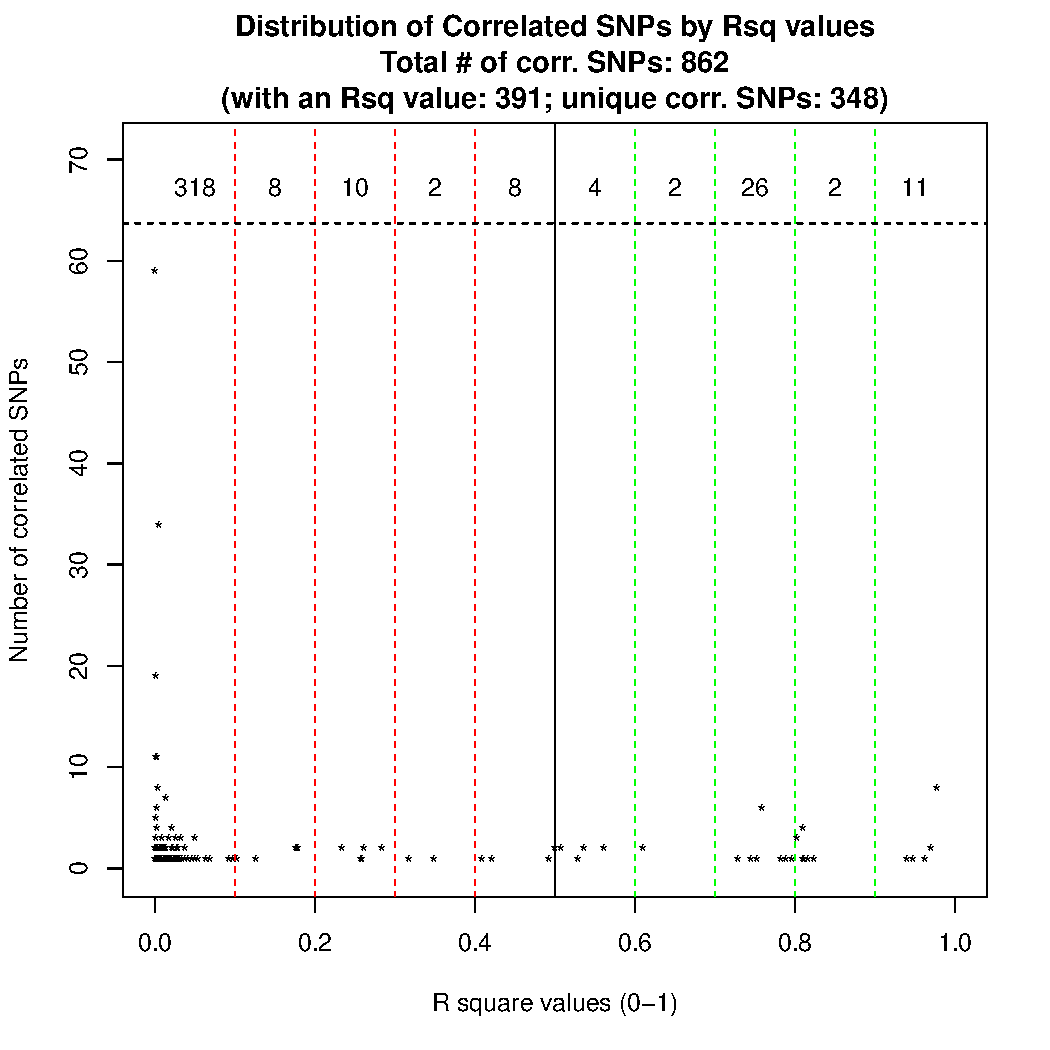
\includegraphics{glioma_dist.pdf}
\caption{\label{fig:glioma_dist.pdf} Distribution of Rsquare values of all 
Correlated SNPs. Each marked bin contains the total number of correlated SNPs. The
 sum of all the counts would total the number of correlated SNPs.}
{\footnotesize{}}
\end{center}
\end{figure}
Using splitbysnp argument, the same type of plot as above (Figure 
        \ref{fig:glioma_dist.pdf}) is generated, however the total number of 
correlated SNPs are divided by the associated tagSNP.
\begin{Schunk}
\begin{Sinput}
> FunciSNPplot(glioma.anno, splitbysnp=TRUE)
> ggsave("glioma_dist_bysnp.pdf")
\end{Sinput}
\end{Schunk}
\begin{figure}[ht!]
\begin{center}
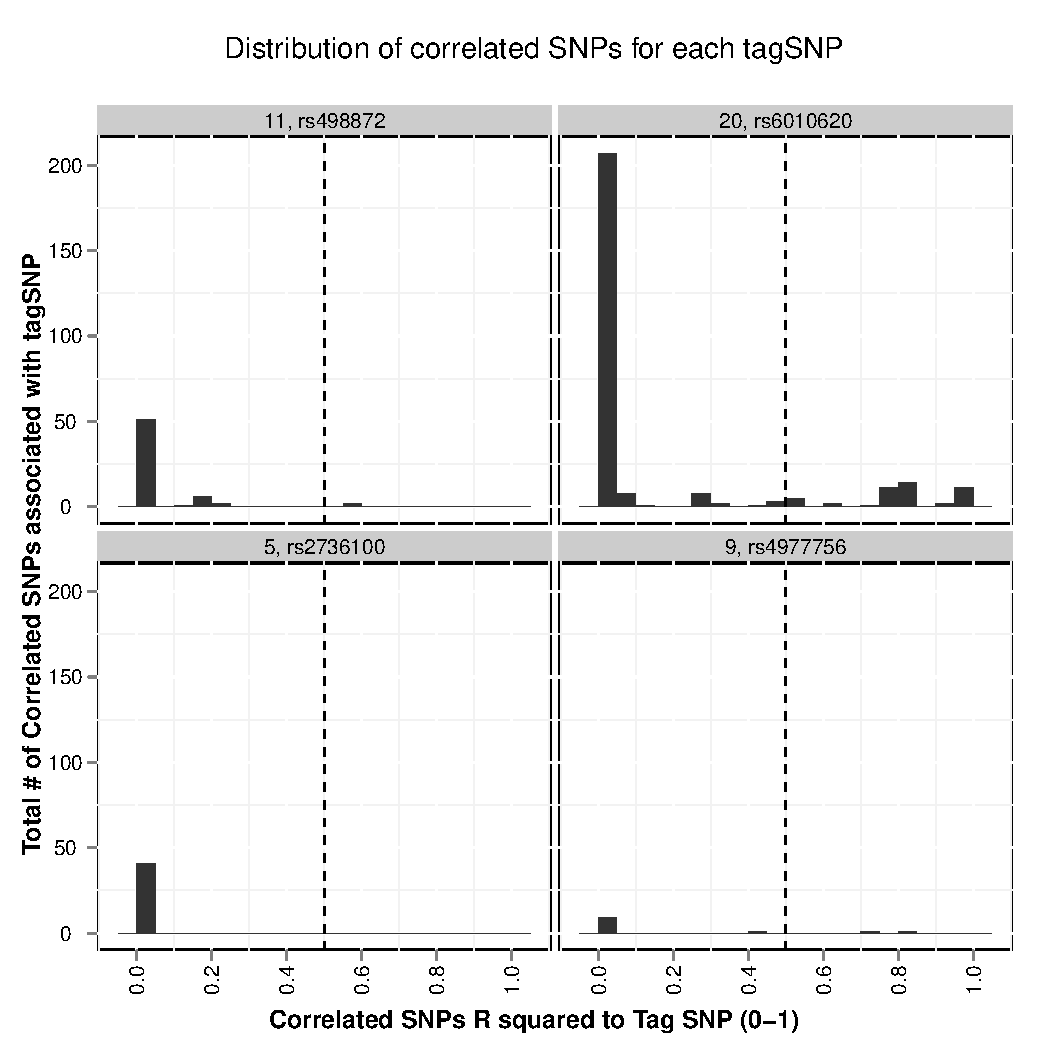
\includegraphics{glioma_dist_bysnp.pdf}
\caption{\label{fig:glioma_dist_bysnp.pdf} Distribution of Rsquare values of all
 Correlated SNPs divided by the tagSNP and it's location.}
{\footnotesize{}}
\end{center}
\end{figure}
Using genomicSum argument set to TRUE will output the overall genomic 
distribution of the newly identified correlated SNPs.  Using 'rsq' value, the 
plot is divided into all correlated SNPs vs subset. This type of plot informs the 
relative enrichment for genomic features.
\begin{Schunk}
\begin{Sinput}
> pdf("glioma_genomic_sum_rcut.pdf")
> FunciSNPplot(glioma.anno, rsq=0.5, genomicSum=TRUE, save=FALSE)
> dev.off()
\end{Sinput}
\begin{Soutput}
X11cairo 
       2 
\end{Soutput}
\end{Schunk}
\begin{figure}[ht!]
\begin{center}
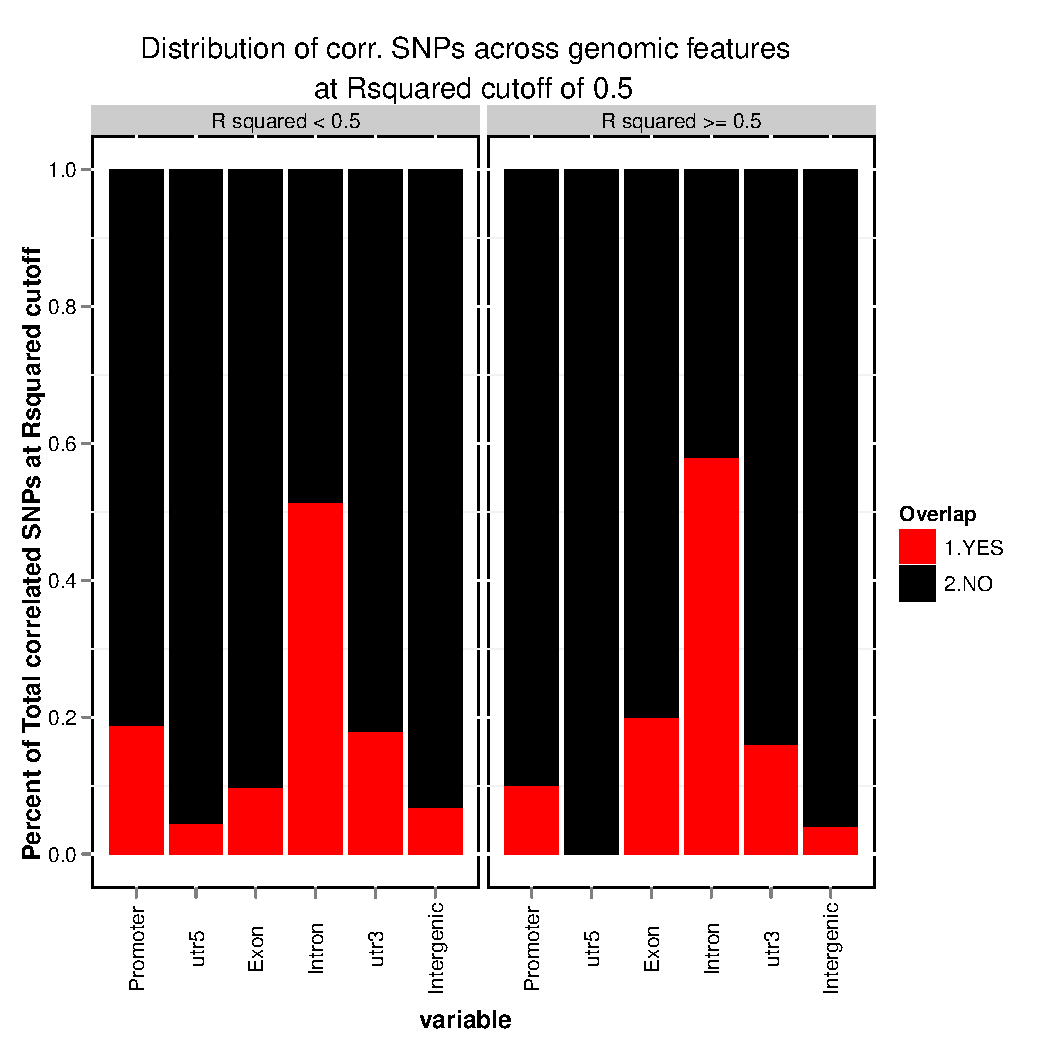
\includegraphics{glioma_genomic_sum_rcut.pdf}
\caption{\label{fig:glioma_genomic_sum_rcut.pdf} Stacked bar chart summarizing 
all correlated SNPs for each of the identified genomie features: exon, intron, 
5UTR, 3UTR, promoter, lincRNA or in gene desert. Rsquare cutoff
 at 0.5. This plot is most informative if used with a rsq value.}
{\footnotesize{}}
\end{center}
\end{figure}
'tagSummary' argument is unique in that it will automatically save all plots in a
specific folder. This is done because this function will generate a summary 
plot for each biofeature.  The first plot (Figure 
        \ref{fig:TFBS_Pol2_U87_R2vsDist_riskSNP.pdf}) is a scatter plot showing 
the relationship between Rsquare and Distance to tagSNP for each FuncySNP. The
 second plot (Figure \ref{fig:TFBS_Pol2_U87_R2summary_riskSNP.pdf}) is a 
 histogram distribution of total number of correlated SNPs at each 
 Rsquare value. This plot is similar to Figure \ref{fig:glioma_dist_bysnp.pdf}, 
 except it is further divided by biofeature. Each set of plot is further divided 
 by tagSNP to help identify locus with the most identifiable FuncySNP. This argument
 is best used in conjunction with a 'rsq' value.
\begin{Schunk}
\begin{Sinput}
> ## Following will output a series of plots for each biofeature at rsq=0.5
> FunciSNPplot(glioma.anno, tagSummary=TRUE, rsq=0.5)
\end{Sinput}
\begin{Soutput}
Finished plotting  1 / 3 
Finished plotting  2 / 3 
Finished plotting  3 / 3 
\end{Soutput}
\end{Schunk}
\begin{figure}[ht!]
\begin{center}
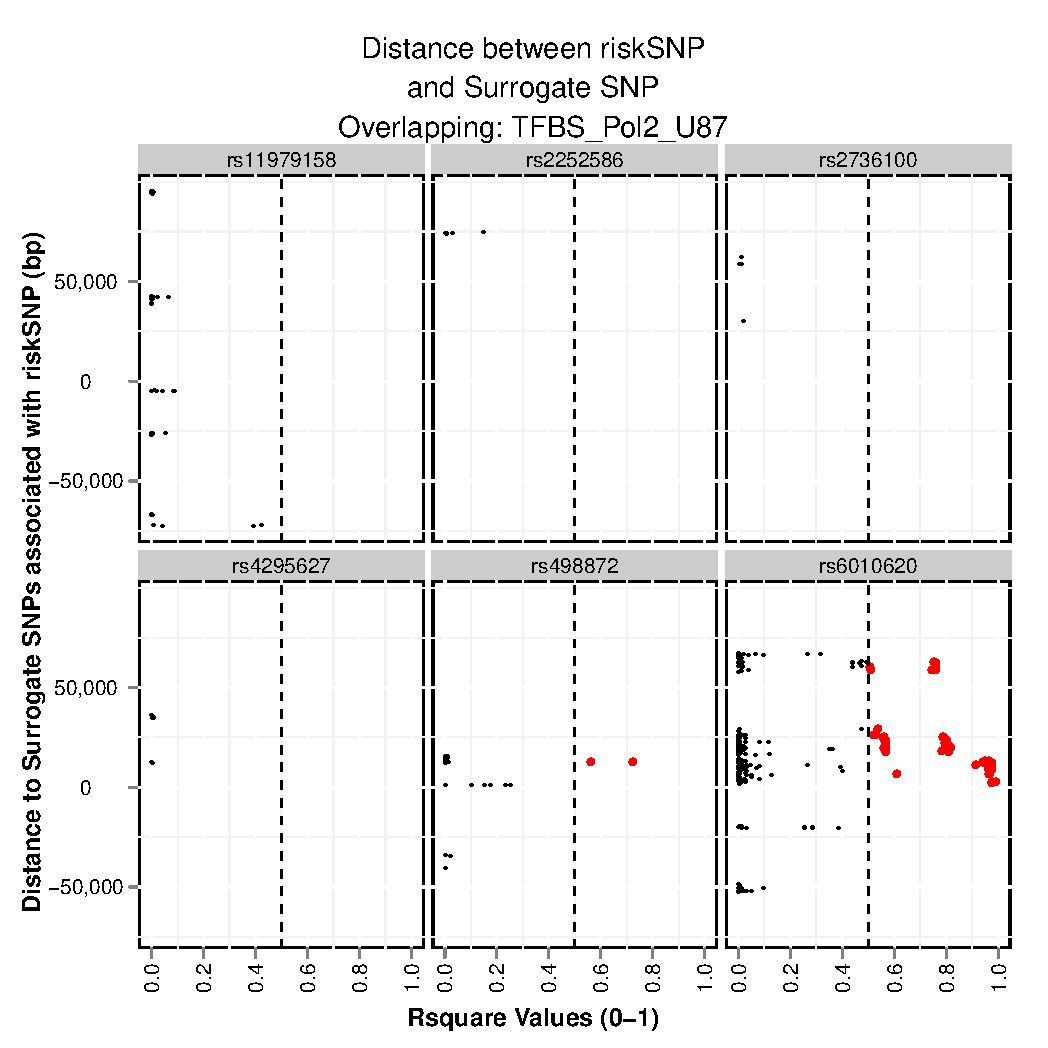
\includegraphics{FunciSNP.0.1.8/plots/TFBS_Pol2_U87_R2vsDist_riskSNP.pdf}
\caption{\label{fig:TFBS_Pol2_U87_R2vsDist_riskSNP.pdf} Scatter plot 
showing the relationship between Rsquare and Distance to tagSNP for each 
FuncySNP}
{\footnotesize{}}
\end{center}
\end{figure}

\begin{figure}[ht!]
\begin{center}
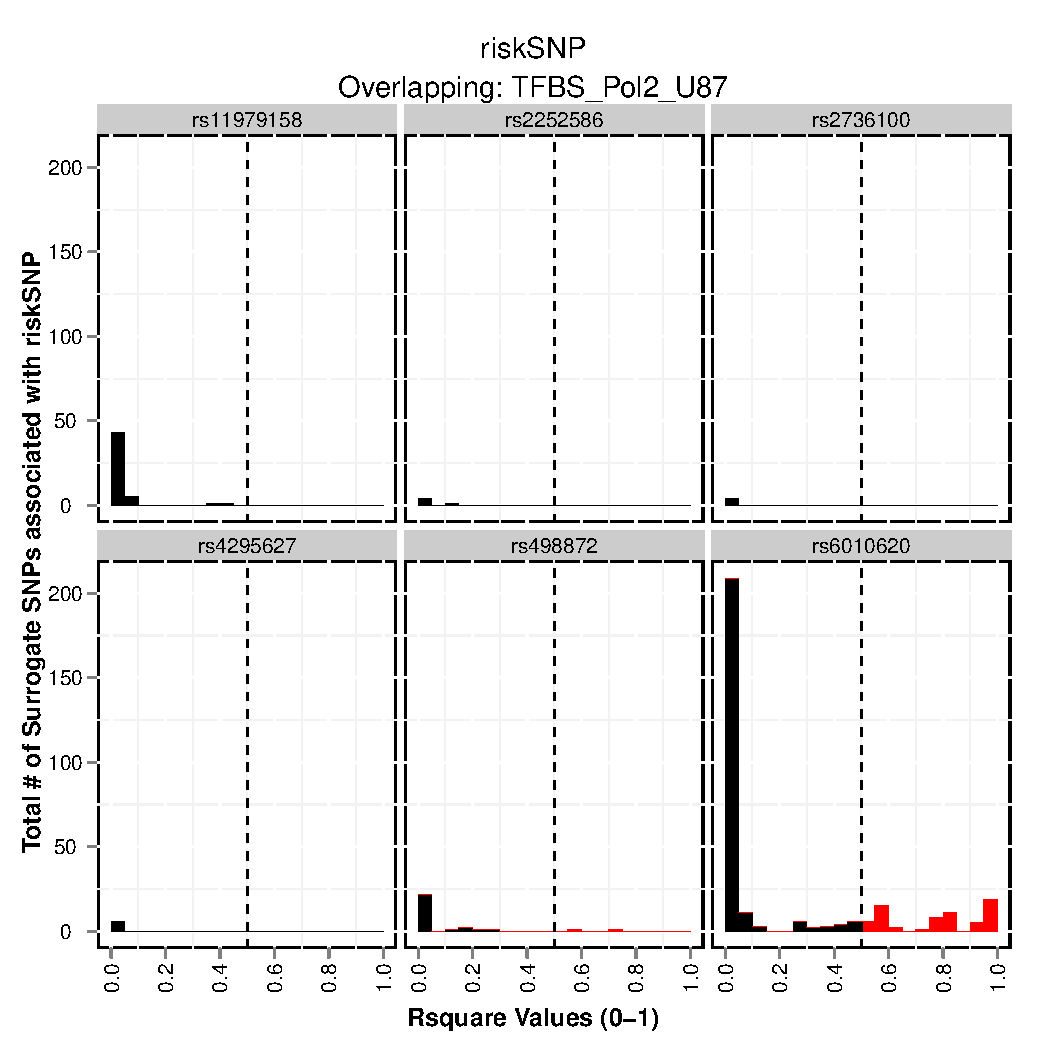
\includegraphics{FunciSNP.0.1.8/plots/TFBS_Pol2_U87_R2summary_riskSNP.pdf}
\caption{\label{fig:TFBS_Pol2_U87_R2summary_riskSNP.pdf} Histogram 
distribution of number of correlated SNPs at each Rsquare value}
{\footnotesize{}}
\end{center}
\end{figure}

\newpage

\subsection*{Output results in BED format - visualize results}
Finally, after evaluating all results using the above tables and plots functions,
 a unique pattern emerges that helps identifies a unique cluster of tagSNP 
 and biofeature that can identify a set of FuncySNPs. To better visualize 
 and to get a better perspective of the location of each newly identified 
 FuncySNP, the results can be outputted using FunciSNPbed.

  FunciSNPbed outputs a unique BED file which can be used to view in any genomic 
browser compatible with BED formats. To learn more about BED formats, see UCSC 
Genome Browser FAQ (http://genome.ucsc.edu/FAQ/FAQformat). Each tagSNP 
which is in LD to a corresponding FuncySNP overlapping at least one biofeature
 is colored black, while the FuncySNP is colored red. The initial position is 
 provided by the first tagSNP and the first linked FuncySNP. We recommend 
 using UCSC genome browser to view your BED files. This is useful so you can 
 view all public and private tracks in relation to FunciSNP results.
\begin{Schunk}
\begin{Sinput}
> ## will output to current working directory.
> FunciSNPbed(glioma.anno, rsq=0.5);
\end{Sinput}
\begin{Soutput}
Total corSNP (RED):  44 
Total tagSNP (BLK):  3 
\end{Soutput}
\begin{Sinput}
> # FunciSNPbed(rs6010620, rsq=0.5);
\end{Sinput}
\end{Schunk}

\newpage

Questions or comments, please contact Simon G. Coetzee (scoetzee NEAR gmail 
 POINT com) or Houtan Noushmehr (houtana NEAR gmail POINT com).

\begin{Schunk}
\begin{Sinput}
> sessionInfo()
\end{Sinput}
\begin{Soutput}
R version 2.14.1 (2011-12-22)
Platform: x86_64-pc-linux-gnu (64-bit)

locale:
 [1] LC_CTYPE=en_US.UTF-8       LC_NUMERIC=C              
 [3] LC_TIME=en_US.UTF-8        LC_COLLATE=en_US.UTF-8    
 [5] LC_MONETARY=en_US.UTF-8    LC_MESSAGES=en_US.UTF-8   
 [7] LC_PAPER=C                 LC_NAME=C                 
 [9] LC_ADDRESS=C               LC_TELEPHONE=C            
[11] LC_MEASUREMENT=en_US.UTF-8 LC_IDENTIFICATION=C       

attached base packages:
 [1] tools     splines   grid      stats     graphics  grDevices utils    
 [8] datasets  methods   base     

other attached packages:
 [1] FunciSNP_0.1.8                         
 [2] VariantAnnotation_1.0.5                
 [3] TxDb.Hsapiens.UCSC.hg19.knownGene_2.6.2
 [4] GenomicFeatures_1.6.7                  
 [5] ChIPpeakAnno_2.2.0                     
 [6] limma_3.10.2                           
 [7] GO.db_2.6.1                            
 [8] BSgenome.Ecoli.NCBI.20080805_1.3.17    
 [9] BSgenome_1.22.0                        
[10] multtest_2.10.0                        
[11] biomaRt_2.10.0                         
[12] GGtools_4.0.0                          
[13] ff_2.2-5                               
[14] bit_1.1-8                              
[15] annotate_1.32.1                        
[16] GGBase_3.14.0                          
[17] genefilter_1.36.0                      
[18] snpStats_1.4.1                         
[19] Matrix_1.0-3                           
[20] lattice_0.20-0                         
[21] survival_2.36-10                       
[22] rtracklayer_1.14.4                     
[23] RCurl_1.9-5                            
[24] Rsamtools_1.6.3                        
[25] Biostrings_2.22.0                      
[26] GenomicRanges_1.6.6                    
[27] IRanges_1.12.5                         
[28] matlab_0.8.9                           
[29] ggplot2_0.8.9                          
[30] proto_0.3-9.2                          
[31] reshape_0.8.4                          
[32] plyr_1.7.1                             
[33] gplots_2.10.1                          
[34] KernSmooth_2.23-7                      
[35] caTools_1.12                           
[36] bitops_1.0-4.1                         
[37] gdata_2.8.2                            
[38] gtools_2.6.2                           
[39] org.Hs.eg.db_2.6.4                     
[40] RSQLite_0.11.1                         
[41] DBI_0.2-5                              
[42] AnnotationDbi_1.16.11                  
[43] Biobase_2.14.0                         

loaded via a namespace (and not attached):
[1] digest_0.5.1    MASS_7.3-16     parallel_2.14.1 XML_3.9-4      
[5] xtable_1.6-0    zlibbioc_1.0.0 
\end{Soutput}
\end{Schunk}

\end{document}
